\chapter{Лабораторная работа №7. Цифровой звук.}

\section{Цифровой звук}

В современном мире цифровая обработка сигналов почти повсеместно вытеснила аналоговую. Исключением не стала и отрасль, относящаяся к записи, хранению и воспроизведению звука. С точки зрения обычного пользователя ещё 20 лет назад были повсеместно распространены аналоговые кассетные проигрыватели, которым на смену пришли уже цифровые CD-диски, затем MP3, а затем, вместе с развитием сети интернет, и стриминговые сервисы.


Чем же отличается цифровой сигнал от аналогового?
\begin{itemize}
	\item Цифровой сигнал дискретен. То есть, в отличие от непрерывного аналогового сигнала, цифровой существует только в те моменты времени, в которые было произведено аналого-цифровое преобразование. Пример аналогового сигнала показан на рисунке \ref{lab7:pic1}. Пример дискретного сигнала показан на рисунке \ref{lab7:pic2}. 
	\item Шкала уровня цифрового сигнала квантованная. В то время, как уровень аналогового сигнала может быть любым (например, 0.1232135346546754775474(5) Вольт), то цифровой сигнал может принимать только уровни, определенные его разрядностью. Если мы используем разрядность цифрового сигнала в 2 бита, то он сможет иметь уровни 0, 1, 2 и 3. Окончательный вид цифрового сигнала показан на рисунке \ref{lab7:pic3}.
\end{itemize}



\begin{figure}[H]
	\centering
	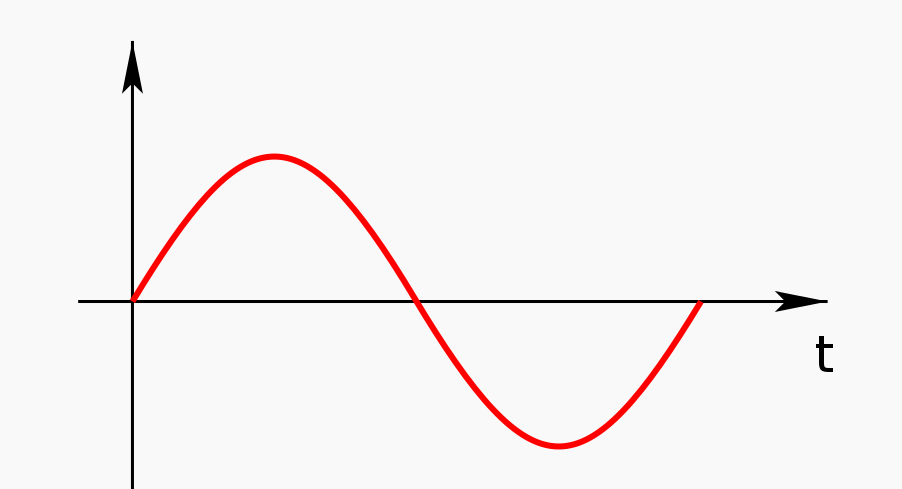
\includegraphics [width=0.7\textwidth] {images/lab_7/analog.png}
	\caption{Форма волны аналогового сигнала.}
	\label{lab7:pic1}
\end{figure}


\begin{figure}[H]
	\centering
	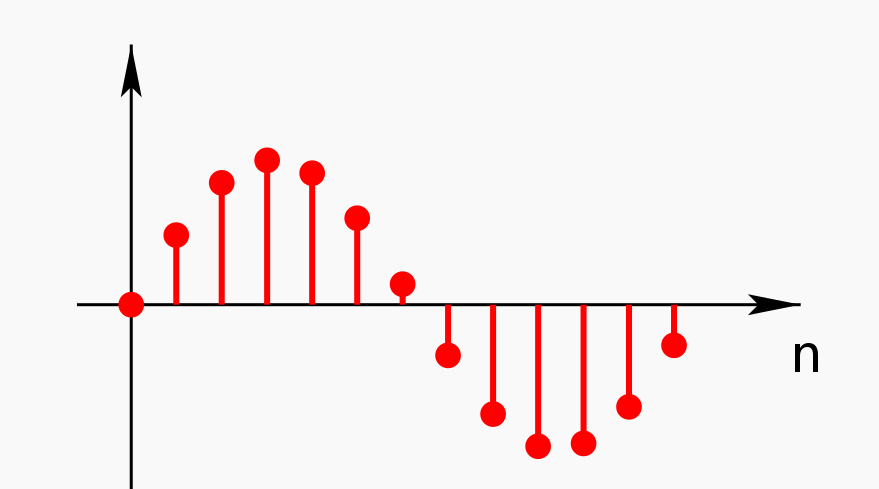
\includegraphics [width=0.7\textwidth] {images/lab_7/discrete.png}
	\caption{Форма волны дискретного сигнала.}
	\label{lab7:pic2}
\end{figure}


\begin{figure}[H]
	\centering
	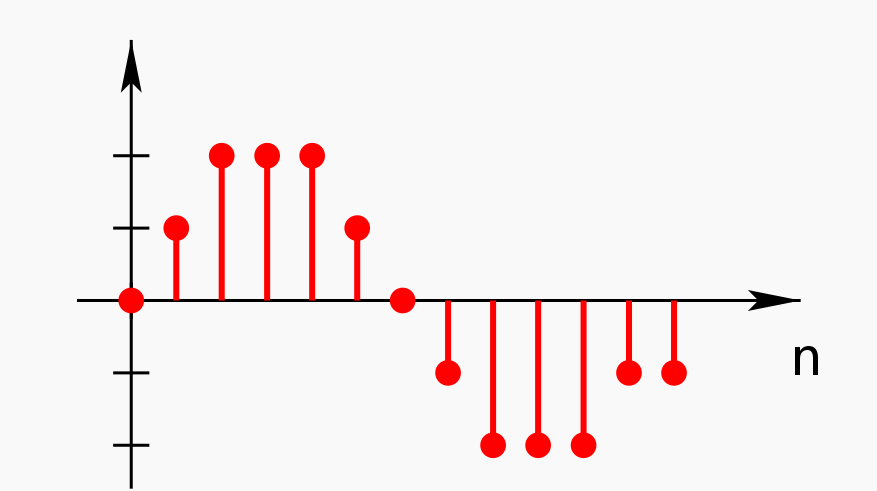
\includegraphics [width=0.7\textwidth] {images/lab_7/digital.png}
	\caption{Форма волны цифрового сигнала (дискретного и квантованного).}
	\label{lab7:pic3}
\end{figure}

Оцифровкой аналогового сигнала называется сочетание двух процессов -- дискретизации и квантования.

Частотой дискретизации цифрового сигнала называется частота, с которой была произведена дискретизация сигнала при аналого-цифровом преобразовании.

Теорема Котельникова (в англоязычной литературе — теорема Найквиста — Шеннона) гласит, что для того, чтобы оцифровать сигнал с максимальной частотой в спектре $f$, необходимо использовать частоту дискретизации $F_s$ как минимум в 2 раза большую, чем частоту $f$.

$$ F_s > 2*f $$

Рассчитаем необходимую частоту дискретизации для человеческого уха.
Слух человека способен воспринимать диапазон частот от 20 Гц до 20 кГц.
Согласно теореме Котельникова (Найквиста -- Шеннона) для оцифровки воспринимаемого человека звуком необходима частота выше, чем 40 кГц. Стандартной частотой для оцифровки звука считается частота 44.1 кГц, использующаяся в Audio CD.


\section{Синтез цифрового звука}

Цифровой звук может не всегда представлять из себя ранее записанный аналоговый сигнал.
Как и любой цифровой сигнал, звук можно синтезировать.
Такая техника повсеместно использовалась в ранних восьмибитных игровых приставках по простой причине -- памяти таких приставок не хватило бы на то, чтобы хранить даже несколько секунд оцифрованного звука.

Рассмотрим техники простейшего синтеза звука на примере игровой приставки Nintendo Entertainment System (NES, Famicom, в в странах СНГ известна как Dendy).

Звуковой чип этой приставки содержал суммарно 5 каналов для генерации звука:

\begin{itemize}
	\item Два частотных канала с прямоугольной формой сигнала, с переменной скважностью (12.5 \%, 25 \%, 50 \%, 75 \%), 16 уровнями громкости и диапазоном частот от 54 Гц до 28 кГц.
	\item Один частотный канал с треугольной формой сигнала, с фиксированной громкостью, поддерживающий частоты от 27 Гц до 56 кГц.
	\item 1 канал белого шума, с 16-ю уровнями громкости, поддерживающий два режима на 16-и заранее запрограммированных частотах. 
	\item 1 канал цифро-аналогового-преобразователя (ЦАП) с разрядностью в 6 бит, позволяющий воспроизводить короткие фрагменты оцифрованного звука (например, ударные инструменты).

\end{itemize}

В рамках данной лабораторной работы мы познакомимся с генератором прямоугольной формы сигнала.

\subsection{Прямоугольная форма сигнала}

Самой простейшей формой звукового сигнала является прямоугольная. Прямоугольный сигнал имеет всего 2 уровня -- высокий и низкий. 


Скважностью (Duty cycle) прямоугольного импульса называют отношение периода сигнала $T$ к длительности импульса $\tau$. Применительно ко звуку, скважность прямоугольного сигнала влияет его характер звучания.

$$ S = \frac{T}{\tau} $$


\begin{figure}[H]
	\centering
	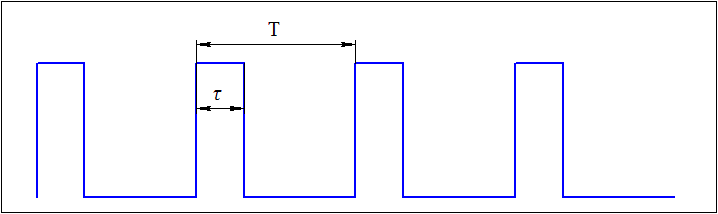
\includegraphics [width=1\textwidth] {images/lab_7/duty_cycle.png}
	\caption{Скважность прямоугольного сигнала.}
	\label{lab7:pic4}
\end{figure}


Опишем входные и выходные порты модуля генерации прямоугольного сигнала.

\noindent
\begin{minipage}{\linewidth}
	\lstinputlisting[language=Verilog, firstline=1, lastline=11]{code_examples/lab_7/square_code.v}
\end{minipage}

\begin{itemize}
	\item Сигнал \textit{enable} управляет генерацией сигнала, позволяет включать и выключать её тогда, когда это нужно.
	\item Сигнал \textit{half\_period} предназначен для управления частотой прямоугольного сигнала. Задаёт полупериод сигнала в тактах clk. Частота прямоугольного сигнала $f$ вычисляется по формуле: 
	$$ f = \frac{F_{clk}}{2* (\textit{half\_period} + 1)} $$
	\item Сигнал \textit{volume} задаёт уровень (громкость) выходного прямоугольного сигнала.

\end{itemize}


Внутренняя логика модуля генерации прямоугольного сигнала основана на простом счётчике. По достижении значения \textit{half\_period} счётчик обнуляется. Счётчик работает только при наличии сигнала \textit{enable}.

\noindent
\begin{minipage}{\linewidth}
	\lstinputlisting[language=Verilog, firstline=12, lastline=22]{code_examples/lab_7/square_code.v}
\end{minipage}

Для хранения непосредственно генерируемой прямоугольной волны добавим одноразрядный регистр square.
При достижении счётчиком значения \textit{half\_period} регистр square инвертируется. Таким образом, формируется прямоугольный сигнал с полупериодом \textit{half\_period}.

\noindent
\begin{minipage}{\linewidth}
	\lstinputlisting[language=Verilog, firstline=24, lastline=33]{code_examples/lab_7/square_code.v}
\end{minipage}

Сформируем выходной сигнал модуля. В случае, если сигналы square и \textit{enable} имеют активный уровень, на выход подаётся значение громкости. В противном случае -- нуль.

\noindent
\begin{minipage}{\linewidth}
	\lstinputlisting[language=Verilog, firstline=35, lastline=36]{code_examples/lab_7/square_code.v}
\end{minipage}

Ниже приведён полный код модуля.

\noindent
\begin{minipage}{\linewidth}
	\lstinputlisting[caption={Код модуля генерации сигнала прямоугольной формы.}, language=Verilog]{code_examples/lab_7/square_code.v}
\end{minipage}


На рисунке \ref{lab7:pic5} показана временная диаграмма работы модуля.

\begin{figure}[H]
	\centering
	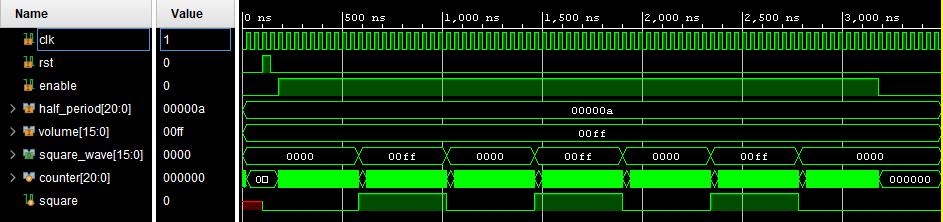
\includegraphics [width=1\textwidth] {images/lab_7/square_simulate.PNG}
	\caption{Временная диаграмма работы модуля генерации сигнала прямоугольной формы.}
	\label{lab7:pic5}
\end{figure}


Представленный дизайн модуля не поддерживает возможность изменения скважности сигнала. Рассмотрим один из способов реализовать данный функционал и сопутствующие изменения логики работы модуля.

Сигнал \textit{half\_period} заменяется парой сигналов \textit{full\_period} и \textit{active\_period}. 

\begin{itemize}
\item \textit{full\_period} обозначает длительность полного периода сигнала (не полупериода, как было ранее) и эквивалентен $T$. Частота сигнала $f$ определяется выражением:
$$ f = \frac{F_{clk}}{\textit{full\_period} + 1} $$ 
\item \textit{active\_period} устанавливает длительность импульса (время, когда прямоугольный сигнал имеет активный уровень) и эквивалентен $\tau$. Скважность сигнала определяется выражением:
$$ S = \frac{\textit{full\_period} + 1}{\textit{active\_period} + 1} $$
\end{itemize}


\noindent
\begin{minipage}{\linewidth}
	\lstinputlisting[language=Verilog, firstline=1, lastline=11]{code_examples/lab_7/square_duty_cycle.v}
\end{minipage}


Verilog-описание счётчика остаётся неизменным, за исключением того, что Сигнал \textit{half\_period} заменён на \textit{full\_period} и, поскольку счётчику придётся отсчитывать в 2 раза больше значений (полный период вместо половины), его разрядность увеличена на 1 бит.

\noindent
\begin{minipage}{\linewidth}
	\lstinputlisting[language=Verilog, firstline=13, lastline=23]{code_examples/lab_7/square_duty_cycle.v}
\end{minipage}


Описание генератора импульсов изменилось. Теперь его работа разбивается на две фазы:
\begin{itemize}
	\item Фаза, когда значение counter меньше, чем \textit{active\_period}. Во время этой фазы значение square выставляется равным единице.
	\item Фаза, когда значение counter больше или равно \textit{active\_period}. Во время этой фазы значение square выставляется равным нулю.
\end{itemize}

\noindent
\begin{minipage}{\linewidth}
	\lstinputlisting[language=Verilog, firstline=25, lastline=36]{code_examples/lab_7/square_duty_cycle.v}
\end{minipage}

На рисунке \ref{lab7:pic6} показана временная диаграмма работы модуля.

\begin{figure}[H]
	\centering
	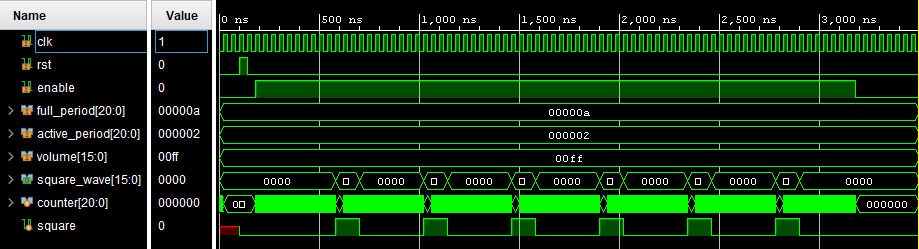
\includegraphics [width=1\textwidth] {images/lab_7/square_simulate2.PNG}
	\caption{Временная диаграмма работы модуля генерации сигнала прямоугольной формы с изменяемой скважностью.}
	\label{lab7:pic6}
\end{figure}

Полный код описания генератора прямоугольных импульсов с переменной скважностью представлен ниже.


\noindent
\begin{minipage}{\linewidth}
	\lstinputlisting[caption={Код модуля генерации сигнала прямоугольной формы с изменяемой скважностью.}, language=Verilog]{code_examples/lab_7/square_duty_cycle.v}
\end{minipage}



\section{Вывод звука на отладочном стенде Terasic DE1}

Отладочный стенд Terasic DE1 оснащён микросхемой-кодеком Wolfson WM8731 для ввода и вывода звука. Кодек поддерживает разрядность звука до 24 бит и частоты дискретизации от 8 кГц до 96 кГц.


В данной лабораторной работе вам будет предоставлен проект DE1\_Audio, содержащий всю логику, необходимую для работы с кодеком.

На рисунке \ref{lab7:pic7} показана структурная схема проекта DE1\_Audio.

\begin{figure}[H]
	\centering
	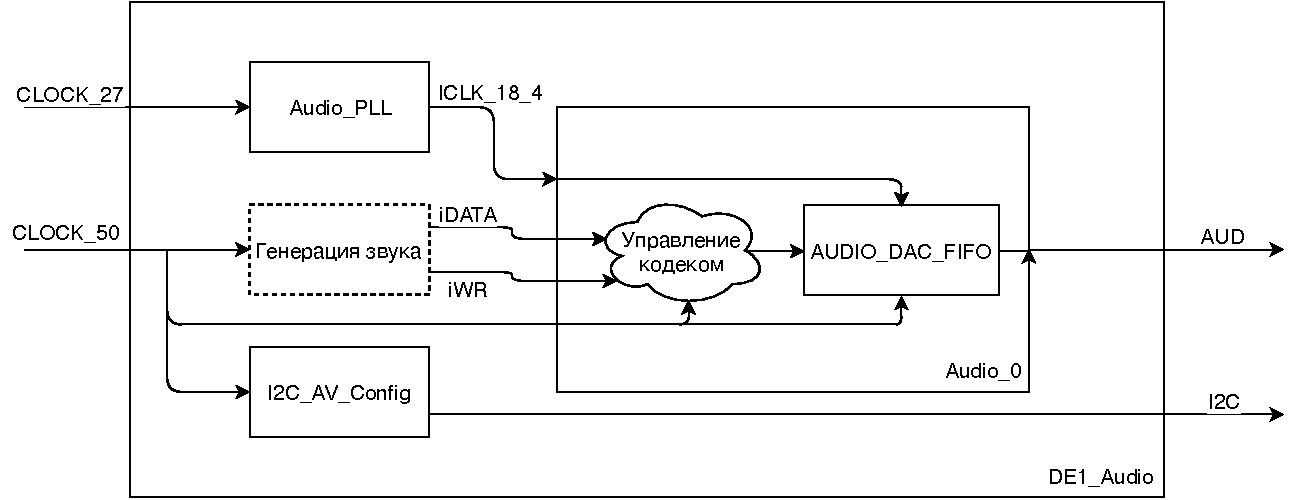
\includegraphics [width=1\textwidth] {images/lab_7/DE1_Audio.pdf}
	\caption{Структурная схема проекта DE1\_Audio.}
	\label{lab7:pic7}
\end{figure}

Проект состоит из следующих модулей:
\begin{enumerate}
	\item Audio\_PLL -- преобразователь частоты на основе ФАПЧ (фазовой автоподстройки частоты). Преобразует частоту входного сигнала \textit{CLOCK\_27} (27 МГц) в сигнал с частотой 18.4 МГц для нужд аудиокодека.
	\item I2C\_AV\_CONFIG -- модуль, производящий первоначальную конфигурацию аудиокодека после подачи сигнала сброса или при загрузке прошивки в ПЛИС.
	\item Audio\_0 -- модуль, включающий в себя логику управления аудиокодеком. Также включает в себя буферное асинхронное FIFO AUDIO\_DAC\_FIFO, предназначенное для выравнивания плотности потока данных и перехода данных из одной тактовой частоты в другую.
	\item Модуль Генерации звука -- модуль, создать который предстоит вам в рамках лабораторной работы. Он должен содержать контроллер PS/2, генератор звуковой волны и управляющий конечный автомат.

\end{enumerate}

Обратите внимание на то, что логика генерации звука должна тактироваться от частоты в 50 МГц.



Для подключения генератора звука к модулю Audio\_0 используются два порта:
\begin{itemize}
	\item \textit{iDATA} -- порт данных (входной относительно Audio\_0) разрядностью 16 бит. В этот порт подаётся поток отчетов звука для дальнейшего преобразования в ЦАП аудиокодека. Обратите внимание, что данные передаются в знаковом формате и старший разряд используется для представления знака. Рекомендуется использовать младшие 15 бит порта.
	\item \textit{iWR} -- порт разрешения на запись данных. Фактически представляет из себя сигнал \textit{write\_enable} для AUDIO\_DAC\_FIFO. При наличии этого сигнала FIFO захватит один отчет данных \textit{iDATA}.

\end{itemize}


Доработаем логику генератора прямоугольной волны без изменяемой скважности, чтобы он генерировал сигнал \textit{iWR}.


%\noindent
%\begin{minipage}{\linewidth}
	\lstinputlisting[caption={Описание модуля генерации прямоугольной волны без изменяемой скважности с сигналом wr.}, language=Verilog]{code_examples/lab_7/square_code_wr.v}
%\end{minipage}


\begin{figure}[H]
	\centering
	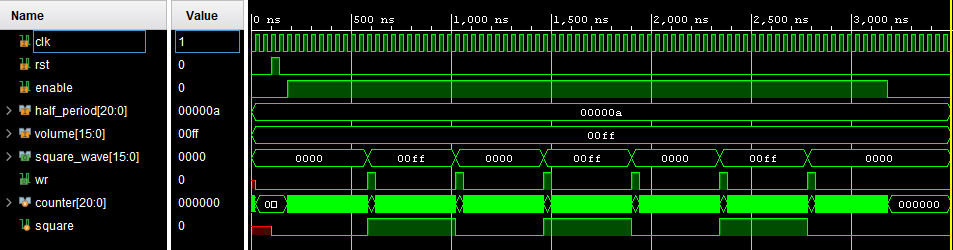
\includegraphics [width=1\textwidth] {images/lab_7/square_simulate3.png}
	\caption{Результат моделирования логики генератора прямоугольной волны без изменяемой скважности с сигналом wr.}
	\label{lab7:pic7}
\end{figure}

\section{Задание лабораторной работы}

Лабораторная работа состоит из двух частей: основной и дополнительной. Задание основной части общее для всех групп и приведено ниже.

\begin{enumerate}
	\item Спроектировать устройство -- музыкальный синтезатор. Синтезатор должен воспроизводить одну из семи нот определенной октавы (согласно варианту) при нажатии на соответствующую цифровую клавишу 1-7 клавиатуры. Форма сигнала -- прямоугольная.
	\item В виду сложности и больших временных затрат на моделирование дизайна целиком, необходимо предоставить результат моделирования только вашего блока.
	\item Ответить на контрольные вопросы.
\end{enumerate}



Вторая часть задания будет выдана непосредственно на лабораторной работе и, с целью исключения обмена исходными кодами, индивидуальна для каждой группы.

\section{Распределение баллов за лабораторную работу}

За основную часть лабораторной работы предполагается начисление максимум 6 баллов.

\begin{enumerate}
\item Посещение
\item Ответы на контрольные вопросы
\item Частично выполненный код лабораторной работы.
\item Полностью выполненный код лабораторной работы
\item Моделирование основной части задания.
\item Полностью работающий проект с основной частью задания.

\end{enumerate}

За дополнительную часть студент может получить от 0 до 8 баллов на усмотрение преподавателя.

С целью экономии времени, студент вправе начать работу сразу над дополнительной частью, минуя основную. По мере выполнения дополнительной части, студент автоматически получит баллы за основную часть.

\section{Контрольные вопросы}

\begin{enumerate}
\item Что такое цифровой звук?
\item Что такое дискретизация?
\item Что такое частота дискретизации?
\item Сформулируйте теорему Котельникова (Найквиста — Шеннона).
\item Что такое квантование?
\item Какие основные формы звукового сигнала вы можете назвать?
\item Как можно синтезировать прямоугольный сигнал?
\item Что такое скважность сигнала?
\end{enumerate}

